\documentclass[tikz]{standalone}

\begin{document}

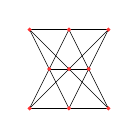
\begin{tikzpicture}
%%% LINES
    \draw[very thin] (0,0) -- (1,0);
    \draw[very thin] (0.5,1) -- (1,0);
    \draw[very thin] (0,0) -- (0.5,1);
    \draw[very thin] (0,1) -- (0.5,0);
    \draw[very thin] (1,1) -- (0.5,0);
    \draw[very thin] (0,1) -- (1,1);
    \draw[very thin] (0,0) -- (1,1);
    \draw[very thin] (0,1) -- (1,0);
    \draw[very thin] (0.25,0.5) -- (0.75,0.5);
%%% POINTS
    \filldraw[red!80] (0,0) circle (0.5pt);
    \filldraw[red!80] (0.5,0) circle (0.5pt);
    \filldraw[red!80] (1,0) circle (0.5pt);
    \filldraw[red!80] (0,1) circle (0.5pt);
    \filldraw[red!80] (0.5,1) circle (0.5pt);
    \filldraw[red!80] (1,1) circle (0.5pt);
    \filldraw[red!80] (0.25,0.5) circle (0.5pt);
    \filldraw[red!80] (0.5,0.5) circle (0.5pt);
    \filldraw[red!80] (0.75,0.5) circle (0.5pt);
\end{tikzpicture}

\end{document}